\documentclass[a4paper, 14pt,russian]{article}
\usepackage[utf8x]{inputenc}
\usepackage[T2A]{fontenc}
\usepackage[russian]{babel}
\usepackage{hyperref}
\usepackage{indentfirst} % включить отступ у первого абзаца
\usepackage{listings}
\usepackage{color}
\usepackage{here}
\usepackage{cmap}          % русский поиск в pdf

\usepackage{times}
\renewcommand{\rmdefault}{ftm}

\usepackage{graphicx}
\graphicspath{{pic/}}
\lstset{inputpath=../listings}

\usepackage{caption}
\renewcommand{\lstlistingname}{Листинг}

\frenchspacing

\usepackage{listings}

\makeatletter
\DeclareRobustCommand{\getlstname}{%
	\begingroup
	% \lstname seems to change hyphens into \textendash
	\def\textendash{-}%
	\filename@parse{\lstname}%
	\texttt{\filename@base.\filename@ext}%
	\endgroup
}
\makeatother


\lstset{
	literate={а}{{\selectfont\char224}}1
	{б}{{\selectfont\char225}}1
	{в}{{\selectfont\char226}}1
	{г}{{\selectfont\char227}}1
	{д}{{\selectfont\char228}}1
	{е}{{\selectfont\char229}}1
	{ё}{{\"e}}1
	{ж}{{\selectfont\char230}}1
	{з}{{\selectfont\char231}}1
	{и}{{\selectfont\char232}}1
	{й}{{\selectfont\char233}}1
	{к}{{\selectfont\char234}}1
	{л}{{\selectfont\char235}}1
	{м}{{\selectfont\char236}}1
	{н}{{\selectfont\char237}}1
	{о}{{\selectfont\char238}}1
	{п}{{\selectfont\char239}}1
	{р}{{\selectfont\char240}}1
	{с}{{\selectfont\char241}}1
	{т}{{\selectfont\char242}}1
	{у}{{\selectfont\char243}}1
	{ф}{{\selectfont\char244}}1
	{х}{{\selectfont\char245}}1
	{ц}{{\selectfont\char246}}1
	{ч}{{\selectfont\char247}}1
	{ш}{{\selectfont\char248}}1
	{щ}{{\selectfont\char249}}1
	{ъ}{{\selectfont\char250}}1
	{ы}{{\selectfont\char251}}1
	{ь}{{\selectfont\char252}}1
	{э}{{\selectfont\char253}}1
	{ю}{{\selectfont\char254}}1
	{я}{{\selectfont\char255}}1
	{А}{{\selectfont\char192}}1
	{Б}{{\selectfont\char193}}1
	{В}{{\selectfont\char194}}1
	{Г}{{\selectfont\char195}}1
	{Д}{{\selectfont\char196}}1
	{Е}{{\selectfont\char197}}1
	{Ё}{{\"E}}1
	{Ж}{{\selectfont\char198}}1
	{З}{{\selectfont\char199}}1
	{И}{{\selectfont\char200}}1
	{Й}{{\selectfont\char201}}1
	{К}{{\selectfont\char202}}1
	{Л}{{\selectfont\char203}}1
	{М}{{\selectfont\char204}}1
	{Н}{{\selectfont\char205}}1
	{О}{{\selectfont\char206}}1
	{П}{{\selectfont\char207}}1
	{Р}{{\selectfont\char208}}1
	{С}{{\selectfont\char209}}1
	{Т}{{\selectfont\char210}}1
	{У}{{\selectfont\char211}}1
	{Ф}{{\selectfont\char212}}1
	{Х}{{\selectfont\char213}}1
	{Ц}{{\selectfont\char214}}1
	{Ч}{{\selectfont\char215}}1
	{Ш}{{\selectfont\char216}}1
	{Щ}{{\selectfont\char217}}1
	{Ъ}{{\selectfont\char218}}1
	{Ы}{{\selectfont\char219}}1
	{Ь}{{\selectfont\char220}}1
	{Э}{{\selectfont\char221}}1
	{Ю}{{\selectfont\char222}}1
	{Я}{{\selectfont\char223}}1
}

\lstdefinestyle{base_listing}{ %
	basicstyle=\footnotesize,       % the size of the fonts that are used for the code
	numbers=left,                   % where to put the line-numbers
	numberstyle=\footnotesize,      % the size of the fonts that are used for the line-numbers
	stepnumber=1,                   % the step between two line-numbers. If it is 1 each line will be numbered
	numbersep=5pt,                  % how far the line-numbers are from the code
	backgroundcolor=\color{white},  % choose the background color. You must add \usepackage{color}
	showspaces=false,               % show spaces adding particular underscores
	showstringspaces=false,         % underline spaces within strings
	showtabs=false,                 % show tabs within strings adding particular underscores
	frame=single,           % adds a frame around the code
	tabsize=2,          % sets default tabsize to 2 spaces
	captionpos=b,           % sets the caption-position to bottom
	breaklines=true,        % sets automatic line breaking
	breakatwhitespace=false,    % sets if automatic breaks should only happen at whitespace
	escapeinside={\%*}{*)},          % if you want to add a comment within your code
	postbreak=\raisebox{0ex}[0ex][0ex]{\ensuremath{\color{red}\hookrightarrow\space}},
	extendedchars=\true
}

\usepackage[left=2.5cm, top=2cm, right=2cm, bottom=2cm, nohead]{geometry}

\begin{document}
\begin{titlepage} % начало титульной страницы

\begin{center} % включить выравнивание по центру

\large Санкт-Петербургский Политехнический Университет Петра Великого\\
\large Институт компьютерных наук и технологий \\
\large Кафедра компьютерных систем и программных технологий\\[6cm]
% название института, затем отступ 4,5см

\huge Защита информации\\[0.5cm] % название работы, затем отступ 0,6см
\large Отчет по лабораторной работе №1\\[0.1cm]
\large Исследование сетевого трафика\\[5cm]
% тема работы, затем отступ 3,7см
\end{center}

\begin{flushright}
\begin{minipage}{0.5\textwidth}
\begin{flushright}
\textbf{Работу выполнил:}

Раскин Андрей

{Группа:} 43501/3\\


\textbf{Преподаватель:} 

Новопашенный Андрей Гелиевич 
\end{flushright}
\end{minipage} % конец врезки
\end{flushright} % конец выравнивания по левому краю

\vfill % заполнить всё доступное ниже пространство

\begin{center}

\large Санкт-Петербург\\
\large \the\year % вывести дату

\end{center} % закончить выравнивание по центру

\thispagestyle{empty} % не нумеровать страницу
\end{titlepage} % конец титульной страницы

\vfill % заполнить всё доступное ниже пространство

\section{Цель работы}
Закрепление навыков работы в программе WireShark и знаний о некоторых сетевых протоколах. 

\section{Программа работы}
При помощи анализатора сетевого трафика WireShark продемонстрировать в сети:
\begin{enumerate}
	
	\item Работу утилиты ping
	\item Работу утилиты tracert
	\item Работу ICMP-протокола в следующих ситуациях:
	\subitem Отправка фрагментированного ping`а,
	\subitem Получение ошибки 3.1 (Destination host unreachable)
	\item Работу ARP-протокола (запрос и ответ);
	\item Работу протокола TCP в следующих ситуациях:
	\subitem Установка соединения,
	\subitem Разрыв соединения,
	\subitem Попытка соединения на отсутствующий порт
\end{enumerate}

\section{Конфигурация компьютера в сети}
\ref{img:system}
\begin{figure}[h]
	\center{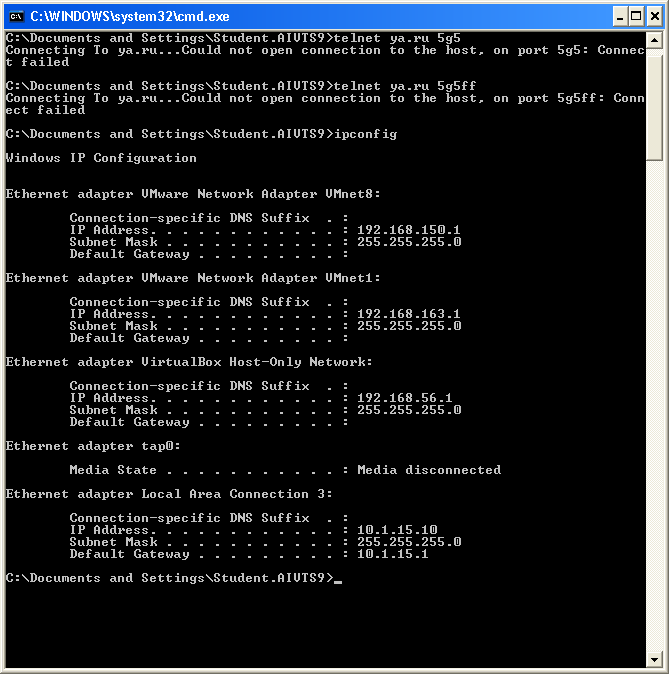
\includegraphics[scale=0.50]{ipconfig}}
	\caption{Конфигурация сети}
	\label{img:system}
\end{figure}

\section{Ход работы}

\subsection{Работы утилиты ping}
	Ping — утилита для проверки целостности и качества соединений в сетях на основе TCP/IP, а также обиходное наименование самого запроса.	Утилита отправляет запросы (ICMP Echo-Request) протокола ICMP указанному узлу сети и фиксирует поступающие ответы (ICMP Echo-Reply). По умолчанию производится 4 попытки отправки запроса.

	\begin{figure}[h!]
		\center{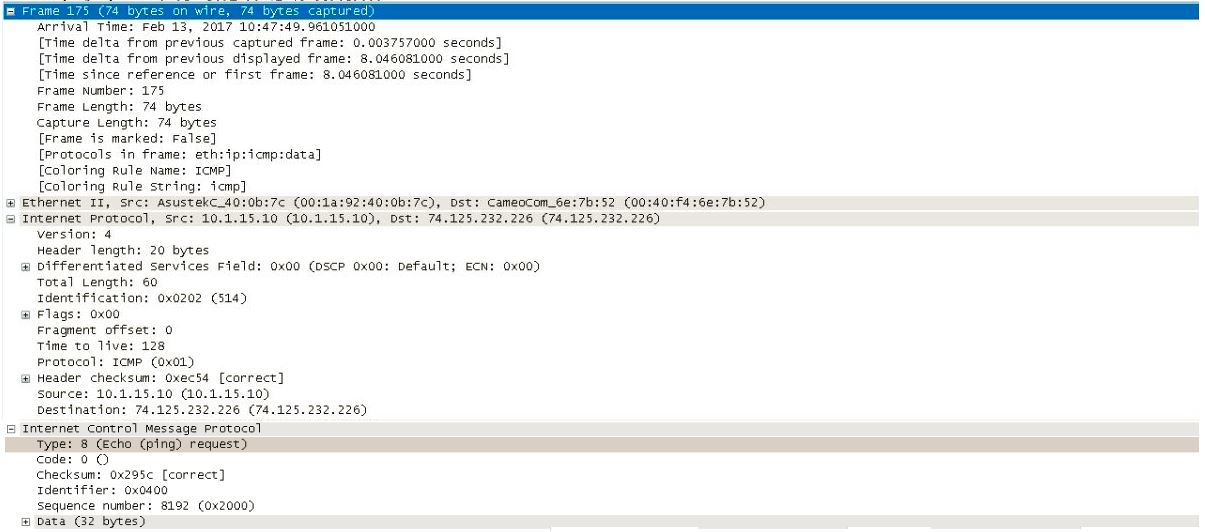
\includegraphics[scale=0.5]{ping}}
		\caption{ICMP эхо запрос}
		\label{img:ping_req}
	\end{figure}

	\begin{figure}[h!]
		\center{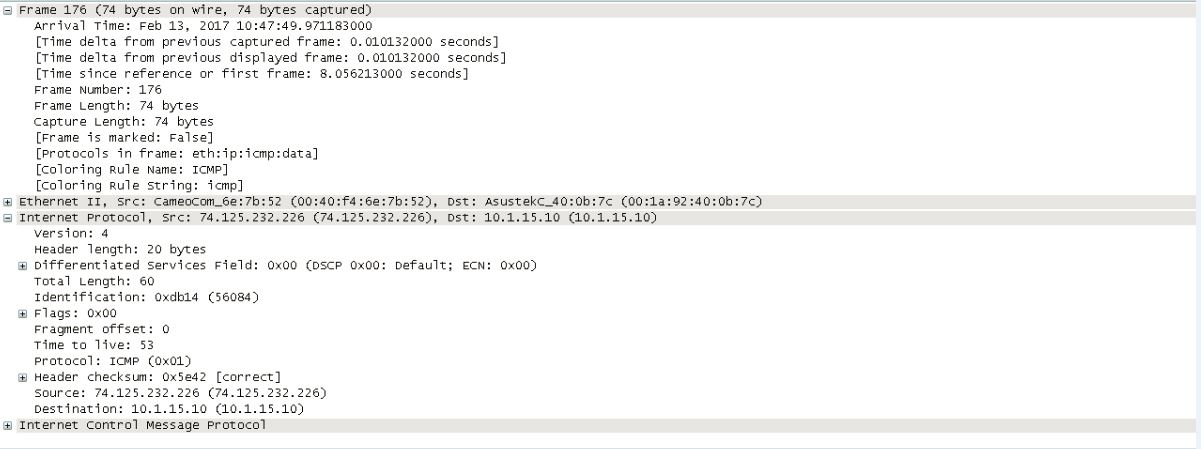
\includegraphics[scale=0.5]{ping2}}
		\caption{ICMP эхо ответ}
		\label{img:ping_ans}
	\end{figure}

	Как видно, в поле Destination указан IP-адрес google.com, поле Source показывает IP-адрес текущего компьютера.
	
\subsection{Работа утилиты tracert}
	В основе работы данной утилиты лежит протокол icmp. Команда TRACERT определяет путь до точки назначения с помощью посылки в точку назначения эхо-сообщений протокола Control Message Protocol (ICMP) с постоянным увеличением значений срока жизни (Time to Live, TTL).
	Попробуем пронаблюдать трассировку маршрута пакетов до узла spbstu.ru при помощи протокола ICMP и утилиты tracert. 

	\begin{figure}[h!]
		\center{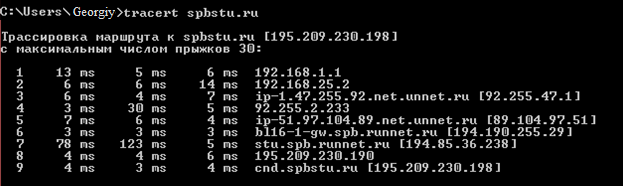
\includegraphics[scale=0.8]{tracert1}}
		\caption{Результат трассировки маршрута в консоли}
		\label{img:tracert1}
	\end{figure}

	\begin{figure}[h!]
		\center{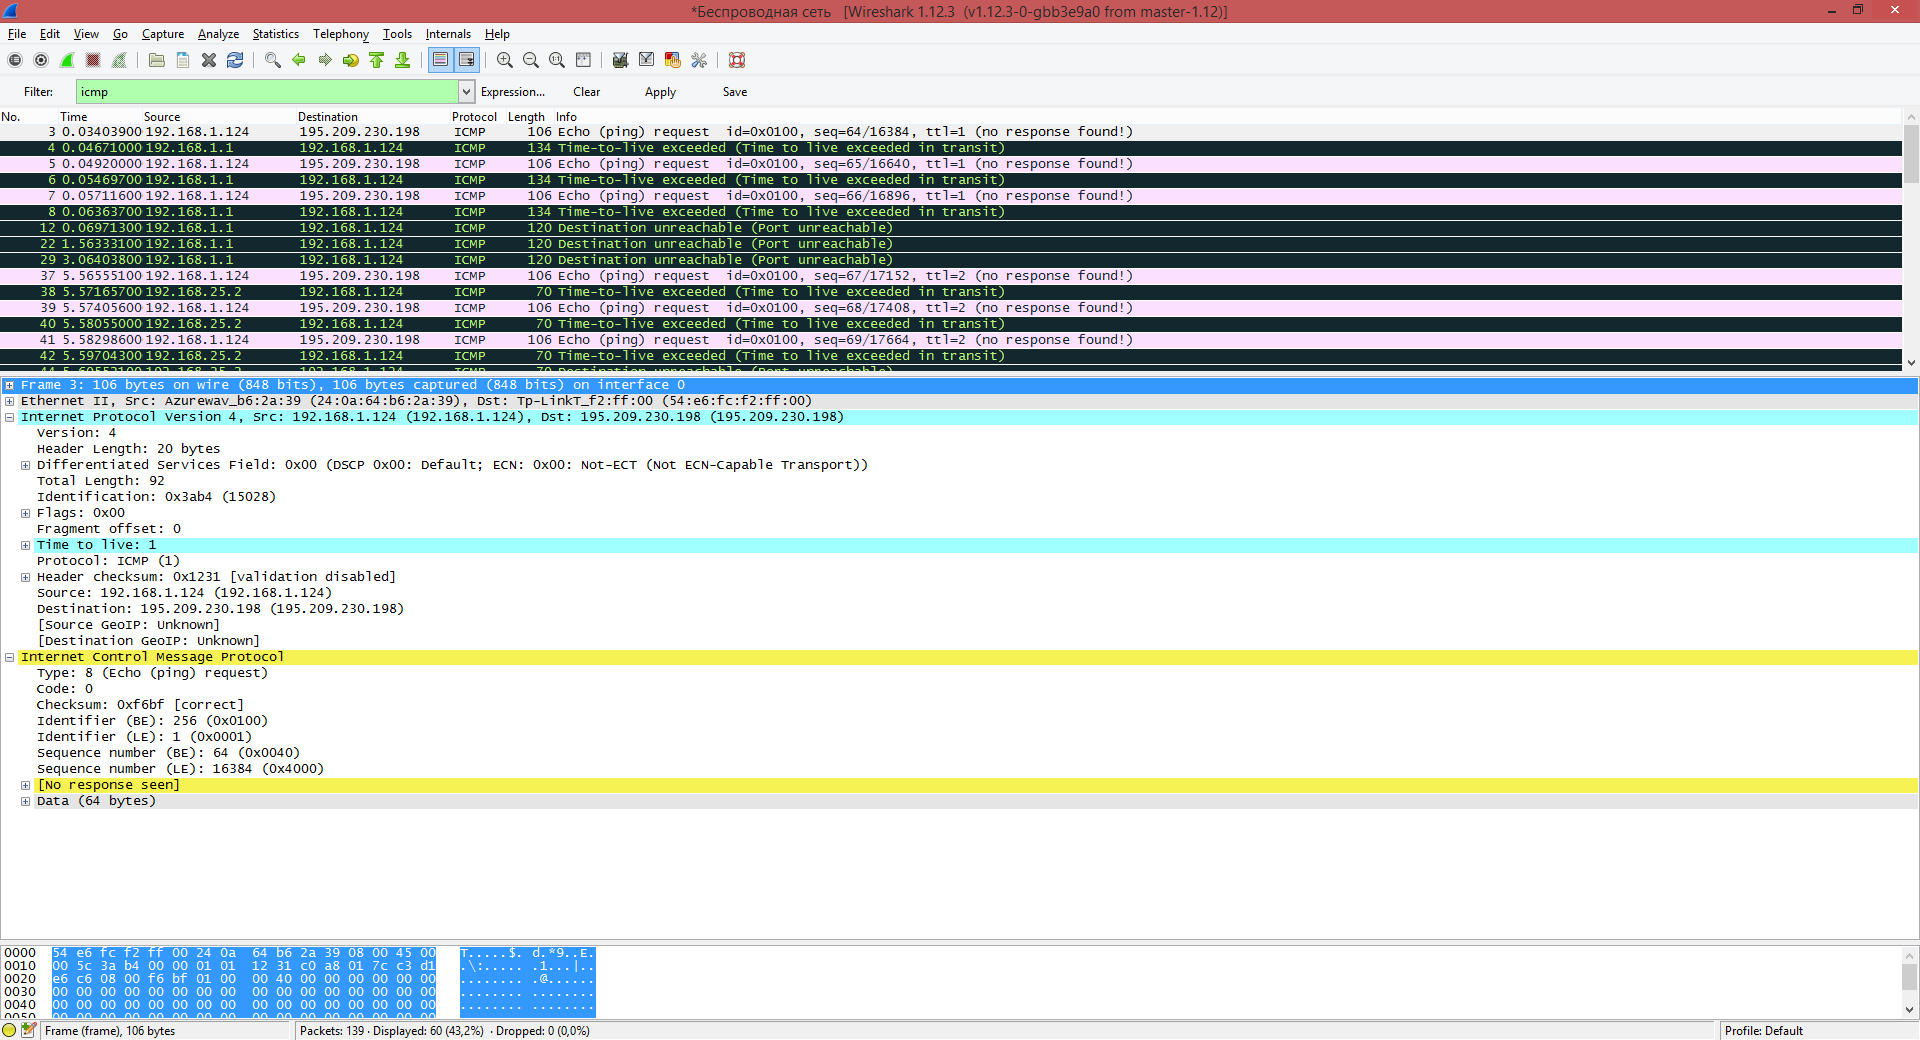
\includegraphics[scale=0.3]{tracert2}}
		\caption{Первый пакет трассировки маршрута}
		\label{img:tracert2}
	\end{figure}
	
	Первый пакет трассировки маршрута отправляется с TTL равным 1. Это значит, что на первом же маршрутизаторе пакет будет уничтожен и нам придет сообщение об ошибке.

	\begin{figure}[h!]
		\center{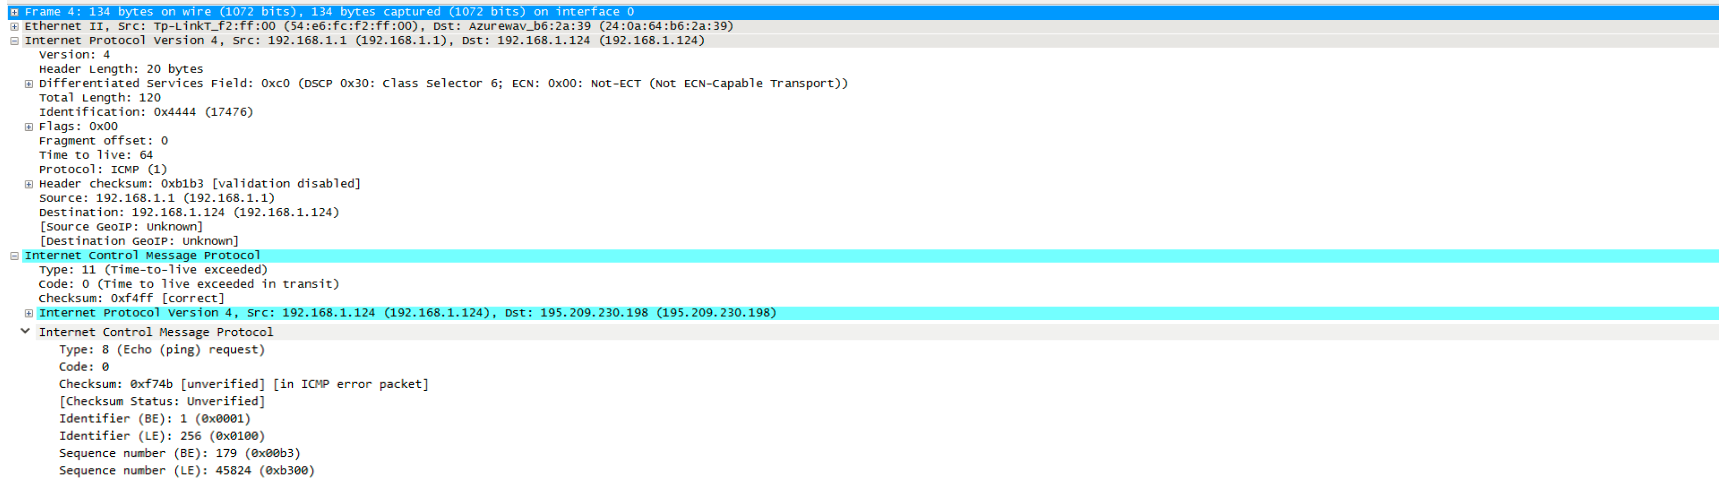
\includegraphics[scale=0.3]{tracert3}}
		\caption{Ответ на первый пакет трассировки}
		\label{img:tracert_ans}
	\end{figure}

	В сообщении об ошибке указан тип ICMP-пакета – 11.0, что означает, что время жизни пакета истекло. Сообщение пришло от маршрутизатора сети, который имеет адрес 192.168.1.1. 
	Аналогично продолжается трассировка маршрута дальше с постепенным инкрементом параметра TTL. Таким образом составляется примерный маршрут прохождения IP-пакета до узла с адресом spbstu.ru.

\subsection{Протокол ICMP}
	\subsubsection{Фрагментированный ping}
		Попробуем отослать фрагментированный ping-запрос. Данный вид запроса использует ICMP-протокол. Для фрагментации пакета необходимо указать его размер, превышающий MTU (maximum transmission unit) - максимальный размер полезного блока данных одного пакета, который может быть передан протоколом без фрагментации. Для протокола Ethernet обычно это чуть больше 1500 байт. Для фрагментации пакета на 3 части укажем размер – 4000 байт.
		
		\begin{figure}[h!]
			\center{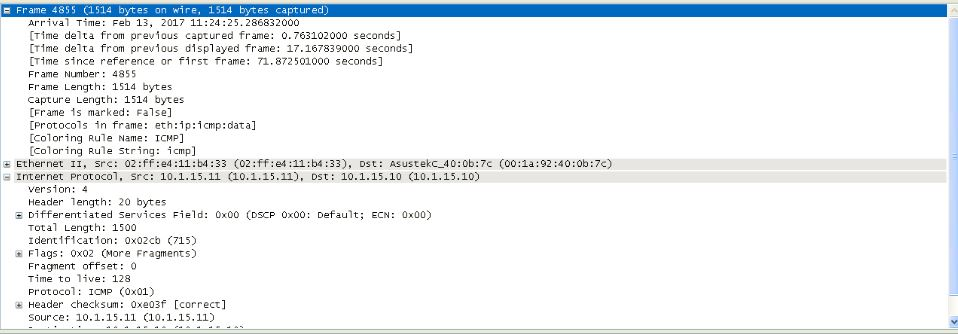
\includegraphics[scale=0.7]{request1}}
			\caption{Ответ на первый пакет трассировки}
			\label{img:frag_ping}
		\end{figure}
	
		О фрагментированности пакета свидетельствуют флаги пакета IP (0x01 – имеются еще фрагменты). О том, что это первый пакет из фрагментированных, свидетельствует нулевое смещение фрагмента. При этом во всех трех IP пакетах содержится ICMP-пакет с одним и тем же идентификатором.
	
	\subsubsection{Несуществующий хост}
	Попробуем пронаблюдать ошибку типа 3.1 (целевой узел недостижим). Для этого отправим ping-запрос на адрес, которого не существует.																																						
	В пакете можно наблюдать типичный ping-запрос (ICMP-пакет типа 8.0).
	\begin{figure}[h!]
		\center{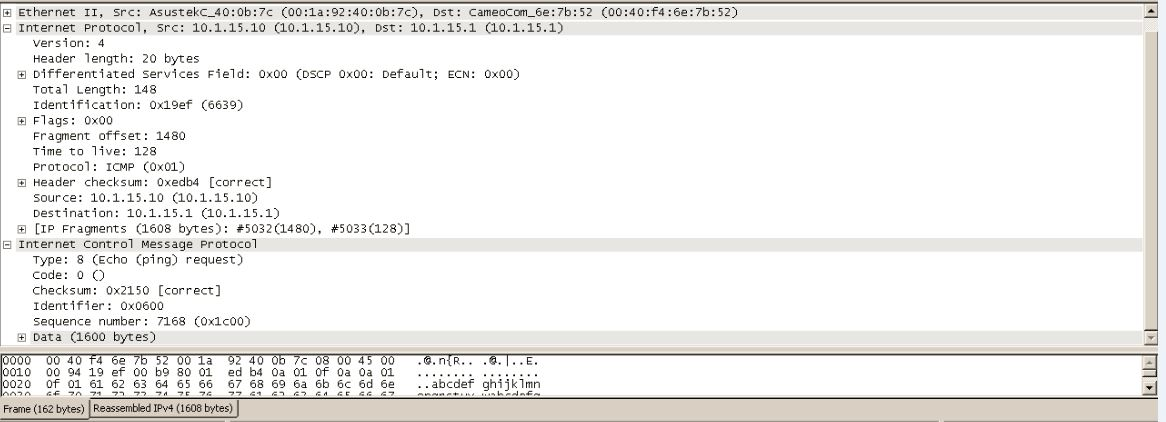
\includegraphics[scale=0.6]{icmp_error}}
		\caption{Ping-запрос}
		\label{img:error_ping}
	\end{figure}

	А вот ответом на указанный выше запрос будет ICMP-пакет типа 3.1, свидетельствующий об ошибке «целевой узел недостижим». При этом, в ответе, в качестве данных пакета отправляется заголовок того пакета, на который пришел ответ.
	\begin{figure}[h!]
		\center{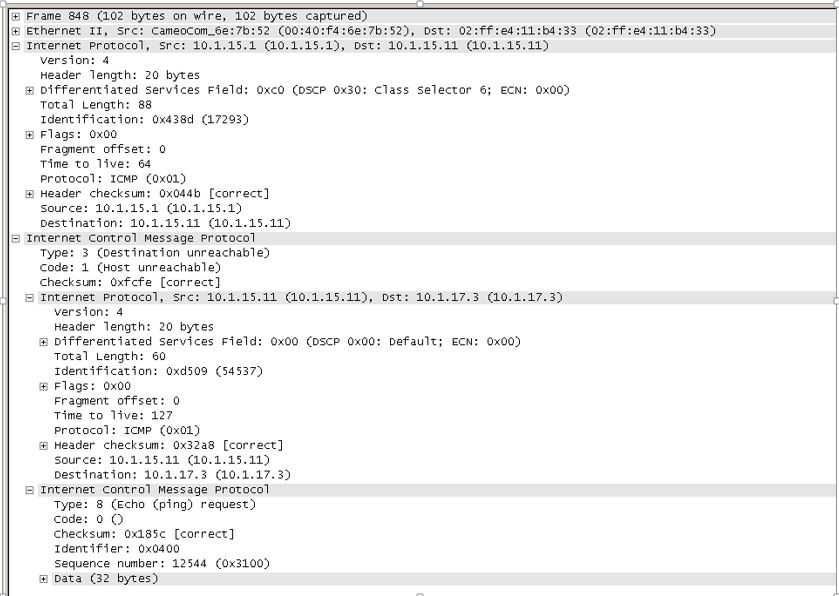
\includegraphics[scale=0.5]{icmp_error2}}
		\caption{ICMP-ответ}
		\label{img:error_ping2}
	\end{figure}

\newpage
\subsection{ARP протокол}
ARP-запрос выполняется по широковещательному адресу (ff:ff:ff:ff:ff:ff), для того, чтобы все узлы сети получили данный пакет. В пакете указывается его тип (поле Opcode) – запрос, а так же целевой IP-адрес для которого запрашивается MAC-адрес. MAC-адрес цели при этом обнулен.
\begin{figure}[h!]
	\center{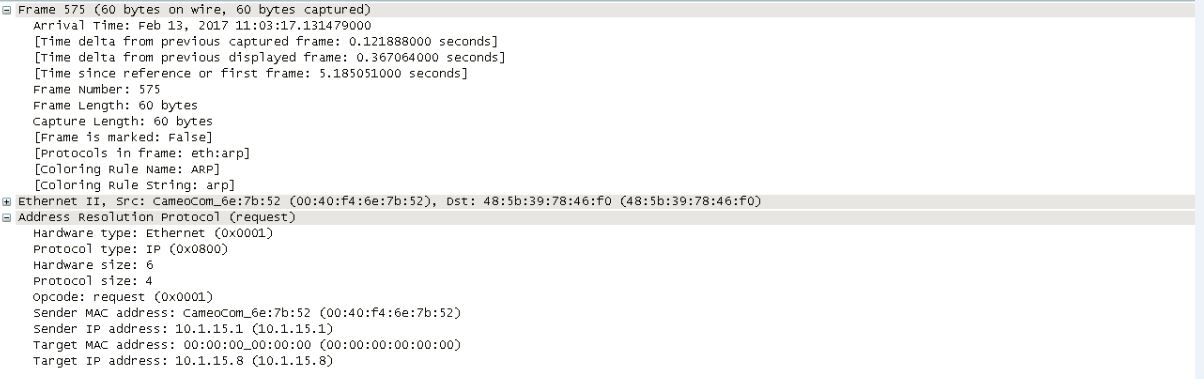
\includegraphics[scale=0.8]{arpR}}
	\caption{Часть IP-пакета, содержащего ARP-запрос}
	\label{img:arp_req}
\end{figure}

\newpage
ARP-ответ отсылается уже на тот адрес, с которого исходил ARP-запрос. В пакете указывается его тип (поле Opcode) – ответ, а так же заполненный MAC-адрес цели.
\begin{figure}[h!]
	\center{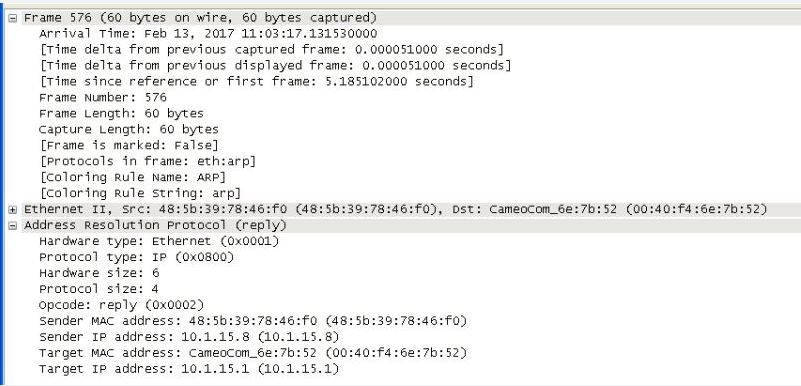
\includegraphics[scale=0.7]{arpA}}
	\caption{Часть IP-пакета, содержащего ARP-ответ}
	\label{img:arp_answ}
\end{figure}

\subsection{TCP-протокол}
	\subsubsection{Установление соединения}
		Эта операция происходит следующим образом: 
		Клиент, посылает серверу сегмент с номером последовательности и флагом SYN.
		\begin{figure}[h!]
			\center{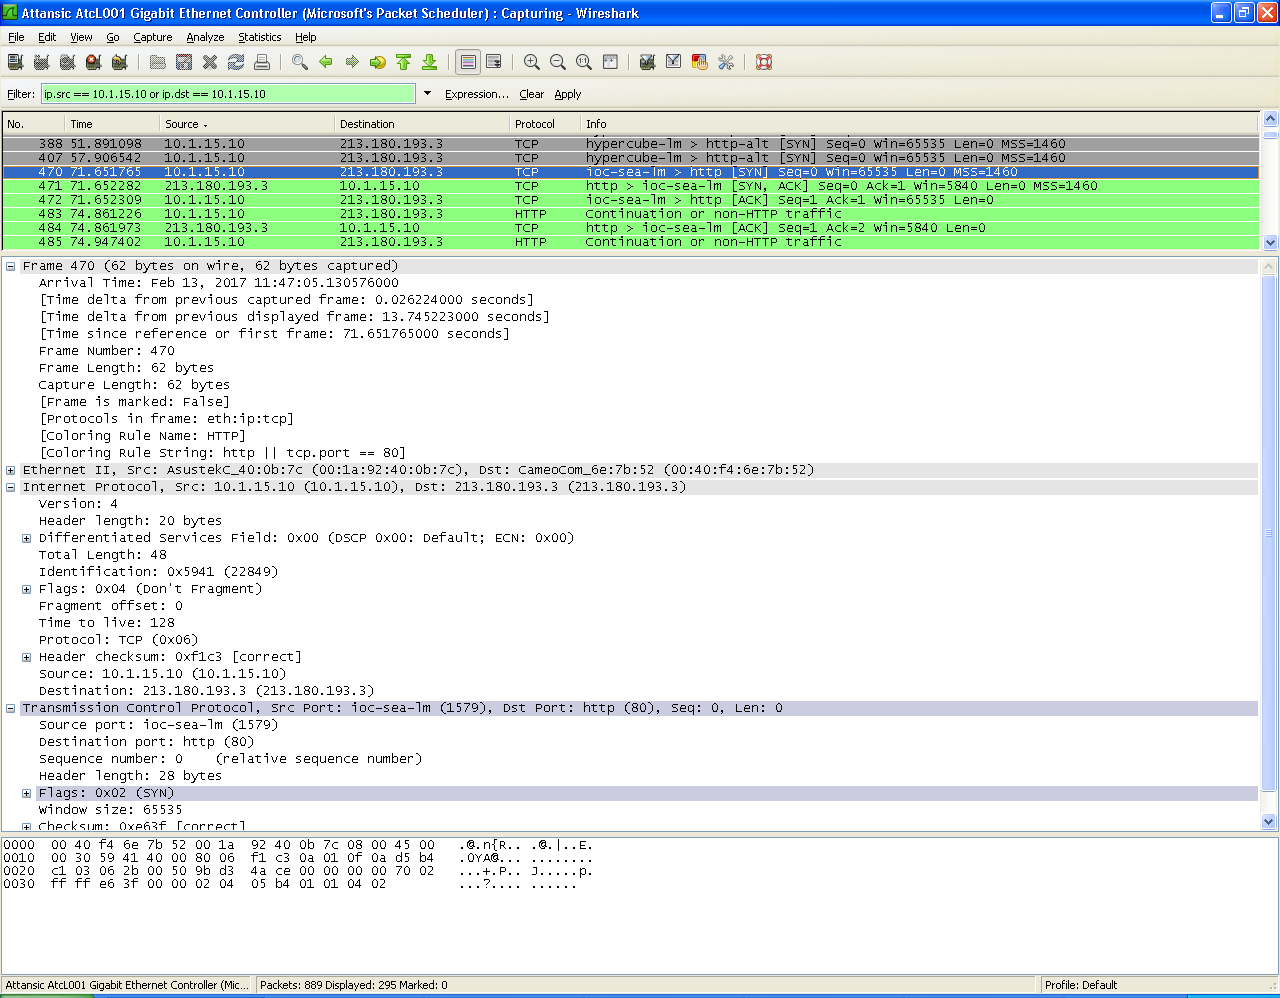
\includegraphics[scale=0.3]{tcp_syn}}
			\caption{TCP запрос на установление соединения SYN}
			\label{img:tcp_syn}
		\end{figure}
		Сервер получает сегмент, запоминает номер последовательности и посылает клиенту сегмент с номером последовательности и флагами SYN и ACK.
		\begin{figure}[h!]
			\center{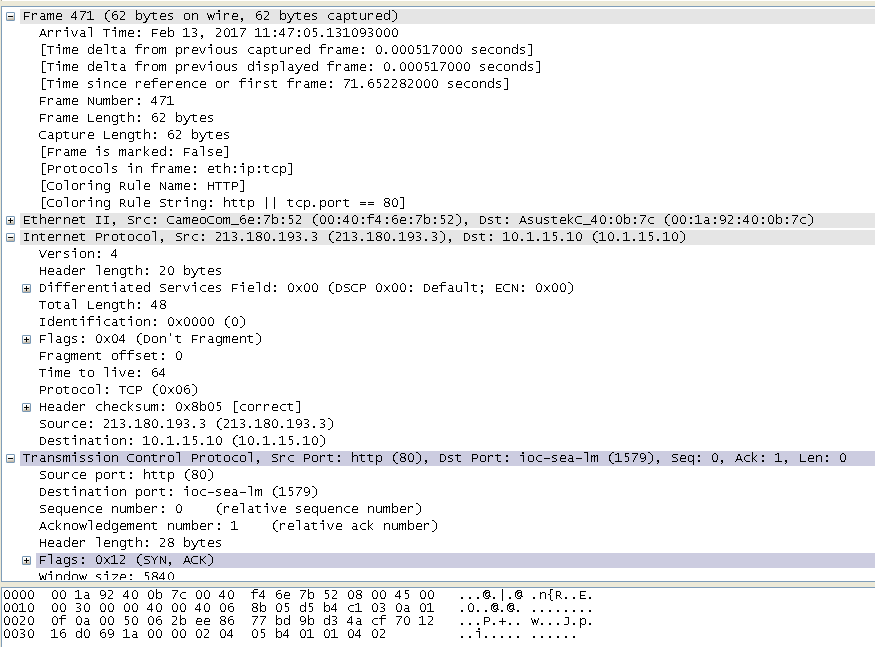
\includegraphics[scale=0.3]{tcp_syn_ack}}
			\caption{Ответ сервера на установление TCP-соединения}
			\label{img:tcp_syn_ack}
		\end{figure}
		Если клиент получает сегмент с флагом SYN, то он запоминает номер последовательности и посылает сегмент с флагом ACK.
		\begin{figure}[h!]
			\center{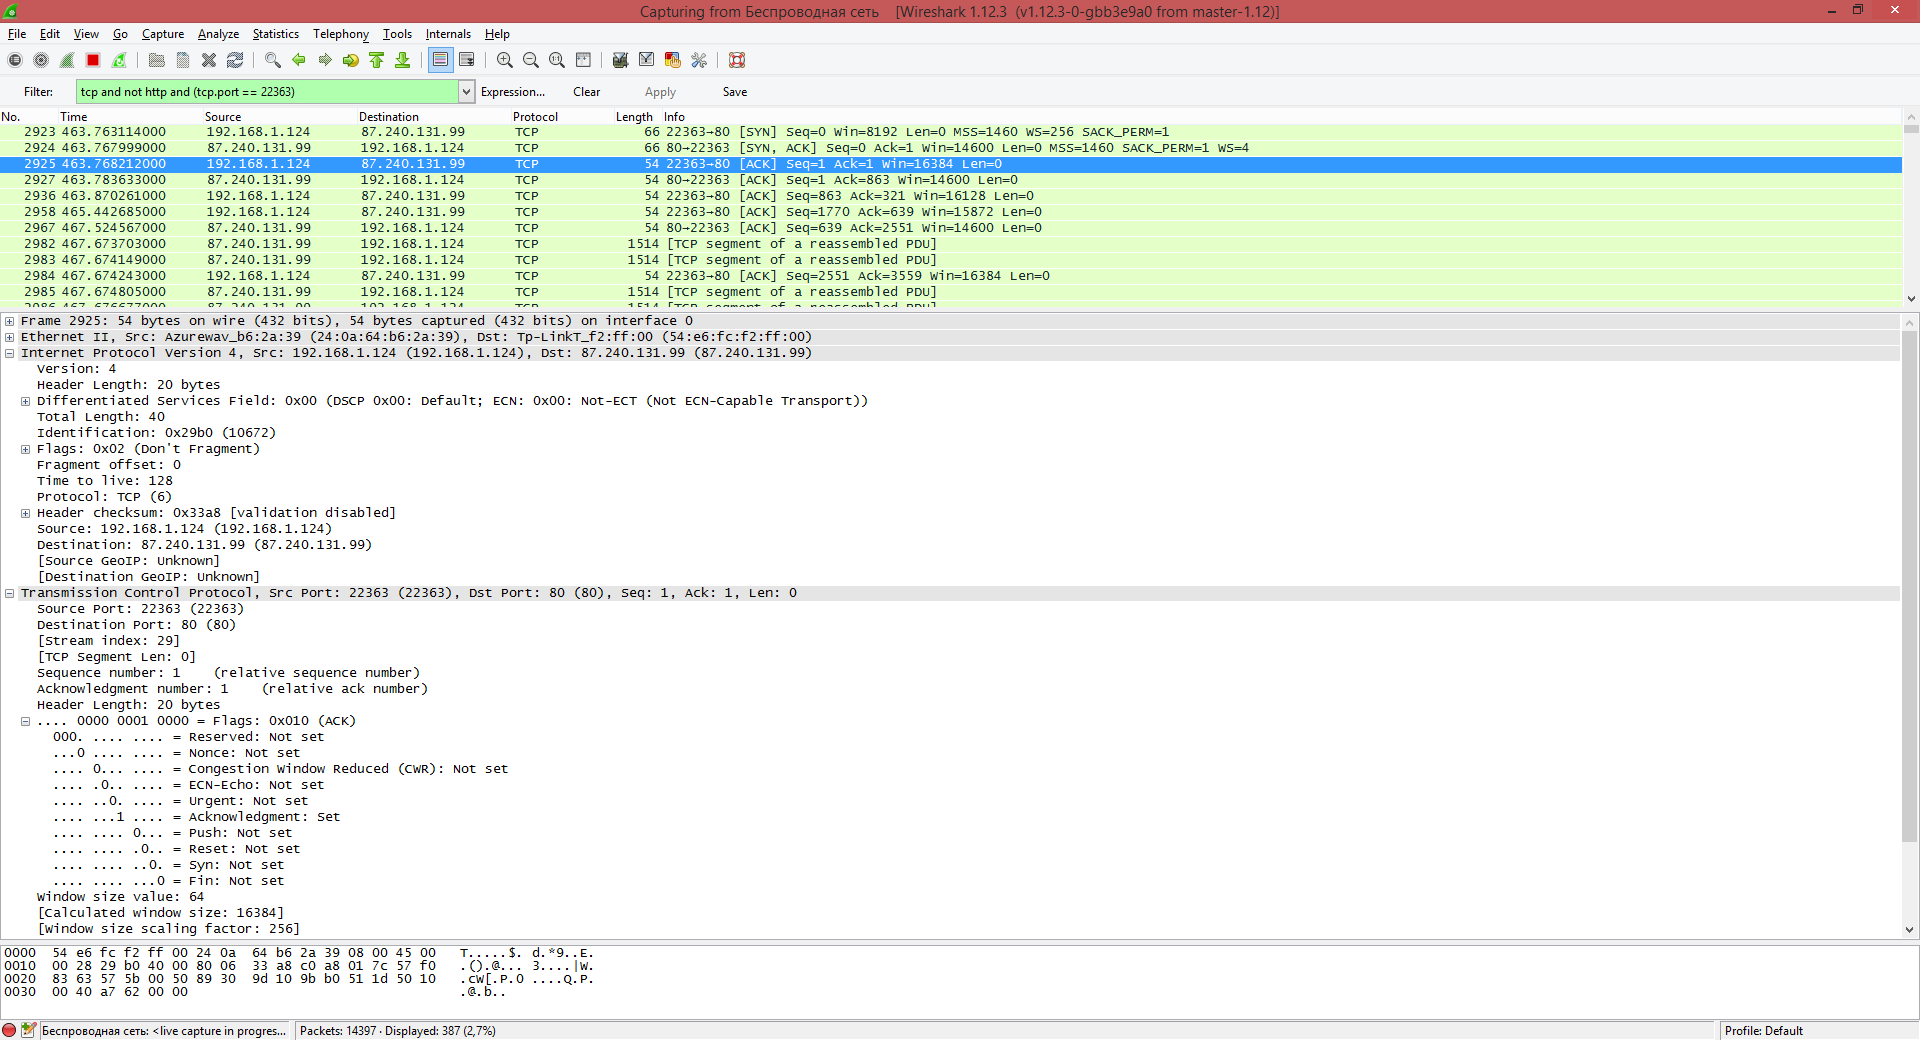
\includegraphics[scale=0.3]{ack}}
			\caption{Подтверждение от клиента о получении ответа}
			\label{img:tcp_ack}
		\end{figure}
	\subsubsection{Разрыв соединения}
		При разрыве соединения сервер отсылает клиенту пакет с установленным флагом RST.
		\begin{figure}[h!]
			\center{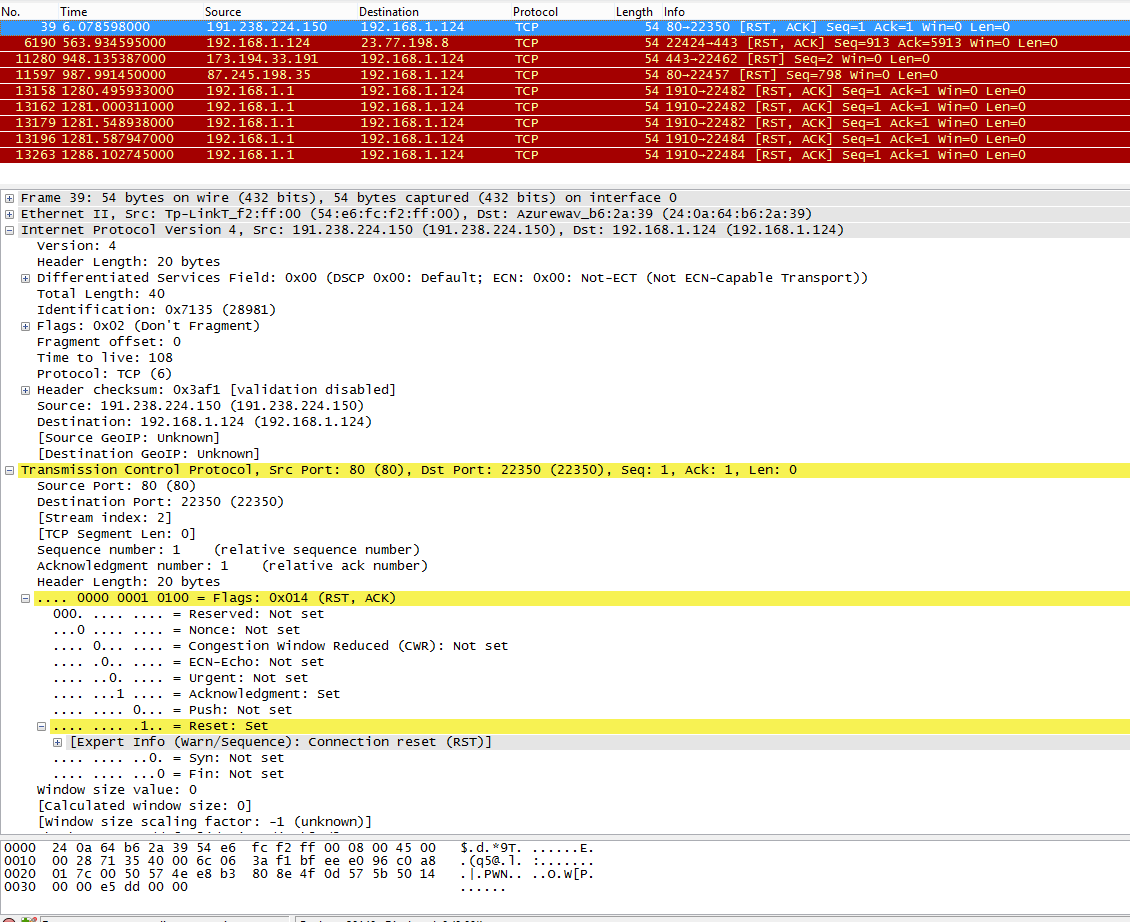
\includegraphics[scale=0.3]{tcp_reset}}
			\caption{Пример пакета с флагом RST}
			\label{img:tcp_reset}
		\end{figure}
	\newpage
	\subsubsection{Установка соединения с отсутствующим портом}
		При попытке подключения к отсутствующему порту, не приходит ACK и RST, поэтому клиент находится в подвешенном состоянии и ожидает ответа.
		\begin{figure}[h!]
			\center{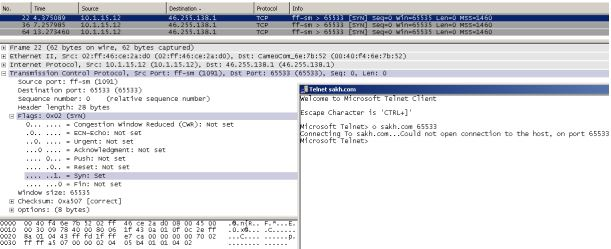
\includegraphics[scale=0.9]{tcp_no}}
			\caption{Пример пакета c подвешенным состоянием}
			\label{img:tcp_reset}
		\end{figure}


\section{Выводы}
В ходе работы были получены навыки работы в программе WireShark и закреплены знания о сетевых протоколах ARP, ICMP, TCP. 
Были рассмотрены: 
\begin{enumerate}
	\item работу утилит ping и tracert;
	\item работа ARP-протокола;
	\item работа протокола ICMP, включая такие типовые случаи, как: отправка фрагментированного пакета, возникновение ошибки 3.1,  трассировка маршрута;
	\item установка, разрыв и завершение TCP соединения;
\end{enumerate}

%\section{Список литературы}
%\begin{itemize}
%	\item Душутина Е.В.  Межпроцессные взаимодействия в операционных системах – СПб, 2014 г, 136 с.
%	\item Душутина Е.В.  Практические вопросы оазработки системных приложений – СПб, 2016 г, 155 с.
%	\item Таненбаум Э., Бос Х. Современные операционные системы. 4-е изд. – СПб.: Питер, 2015 – 1120 с.
%\end{itemize}

\end{document}

